\documentclass[11pt, nohyper, final]{uhrevthesis}
% \documentclass[11pt, nohyper, draft]{uhrevthesis}

\UHRevThesisSetup{
  % Title information:
  title={Sample Thesis Title - Long, Wide, and Words Capitalized},
  author={Maya K. Student},
  dissertation,  % Choose from: thesis, dissertation
  degree={},  % Use default value if left blank
  department={Electrical and Computer Engineering},
  college={Cullen College of Engineering},
  submitdate={},  % Use today if left blank.
  copyrightyear={},  % Use this year if left blank.
  % Whether to print out optional pages:
  lstoftable, lstoffigure, copyright,
  % lstoffigurefirst,  % Will make Lst of Figures before Lst of Tables.
  % titlebold,  % Will make the title font bold.
  % sectitlestyle={title},  % Style of section titles, can be "title", "upper" or "normal".
  % Professor (Committee member) List:
  chair={Name of Chair Professor},  % Required
  cochair={},  % Optional, can be blank
  firstreader={Name of Prof1},  % Required
  secondreader={Name of Prof2},  % Required
  thirdreader={Name of Prof3},  % Optional, can be blank
  fourthreader={Name of Prof4},  % Optional, can be blank
  fifthreader={},  % Optional, can be blank,
  ownerPass={}, userPass={}  % Can be configured only when using XeLaTeX
}

\submitdate{\monthyeardate\formatdate{14}{12}{2022}}
\graphicspath{{pics}}

\begin{document}

\makecoverpages

\begin{dedication}
  \textit{Four score and seven years ago our fathers brought forth on this continent, a new nation, conceived in Liberty, and dedicated to the proposition that all men are created equal.}
  
  \textit{Now we are engaged in a great civil war, testing whether that nation, or any nation so conceived and so dedicated, can long endure. We are met on a great battle-field of that war. We have come to dedicate a portion of that field, as a final resting place for those who here gave their lives that that nation might live. It is altogether fitting and proper that we should do this.}
  
  \textit{But, in a larger sense, we can not dedicate -- we can not consecrate -- we can not hallow -- this ground. The brave men, living and dead, who struggled here, have consecrated it, far above our poor power to add or detract. The world will little note, nor long remember what we say here, but it can never forget what they did here. It is for us the living, rather, to be dedicated here to the unfinished work which they who fought here have thus far so nobly advanced. It is rather for us to be here dedicated to the great task remaining before us -- that from these honored dead we take increased devotion to that cause for which they gave the last full measure of devotion -- that we here highly resolve that these dead shall not have died in vain -- that this nation, under God, shall have a new birth of freedom -- and that government of the people, by the people, for the people, shall not perish from the earth.}
  
  \begin{flushright}
    Abraham Lincoln \\
    \usdate\formatdate{19}{11}{1863}
  \end{flushright}
\end{dedication}


\begin{acknowledgements}
  \singlespacing{
    Lorem ipsum dolor sit amet, consectetur adipiscing elit, sed do eiusmod tempor incididunt ut labore et dolore magna aliqua. Mi proin sed libero enim sed faucibus turpis in eu. Feugiat vivamus at augue eget arcu dictum. Sit amet dictum sit amet justo donec. Vitae nunc sed velit dignissim sodales ut eu sem integer. Aliquam etiam erat velit scelerisque in dictum non consectetur a. Et sollicitudin ac orci phasellus egestas tellus. Maecenas pharetra convallis posuere morbi leo urna molestie. Erat nam at lectus urna duis convallis. Turpis egestas sed tempus urna.
  }
\end{acknowledgements}


\begin{abstract}
  Lorem ipsum dolor sit amet, consectetur adipiscing elit, sed do eiusmod tempor incididunt ut labore et dolore magna aliqua. Mi proin sed libero enim sed faucibus turpis in eu. Feugiat vivamus at augue eget arcu dictum. Sit amet dictum sit amet justo donec. Vitae nunc sed velit dignissim sodales ut eu sem integer. Aliquam etiam erat velit scelerisque in dictum non consectetur a. Et sollicitudin ac orci phasellus egestas tellus. Maecenas pharetra convallis posuere morbi leo urna molestie. Erat nam at lectus urna duis convallis. Turpis egestas sed tempus urna.
\end{abstract}


\makecontentspages

\pagenumbering{arabic}

\sectionalt{Introduction}

Lorem Ipsum is simply dummy text of the printing and typesetting industry. Lorem Ipsum has been the industry's standard dummy text ever since the 1500s, when an unknown printer took a galley of type and scrambled it to make a type specimen book \cite{gridftp}. It has survived not only five centuries, but also the leap into electronic typesetting, remaining essentially unchanged. It was popularised in the 1960s with the release of Letraset sheets containing Lorem Ipsum passages, and more recently with desktop publishing software like Aldus PageMaker including versions of Lorem Ipsum.
\begin{enumerate}
  \item
  List item 1 that tabulates the information
  \item
  Second list item
  \item
  Another list item
  \item
  last list item
\end{enumerate}

Contrary to popular belief, Lorem Ipsum is not simply random text. It has roots in a piece of classical Latin literature from 45 BC, making it over 2000 years old. Richard McClintock, a Latin professor at Hampden-Sydney College in Virginia, looked up one of the more obscure Latin words, consectetur, from a Lorem Ipsum passage, and going through the cites of the word in classical literature, discovered the undoubtable source. Lorem Ipsum comes from sections 1.10.32 and 1.10.33 of "de Finibus Bonorum et Malorum" (The Extremes of Good and Evil) by Cicero, written in 45 BC. This book is a treatise on the theory of ethics, very popular during the Renaissance. The first line of Lorem Ipsum, "Lorem ipsum dolor sit amet..", comes from a line in section 1.10.32.

The standard chunk of Lorem Ipsum used since the 1500s is reproduced below for those interested. Sections 1.10.32 and 1.10.33 from "de Finibus Bonorum et Malorum" by Cicero are also reproduced in their exact original form, accompanied by English versions from the 1914 translation by H. Rackham.

\begin{figure}[ht]
  \begin{center}
    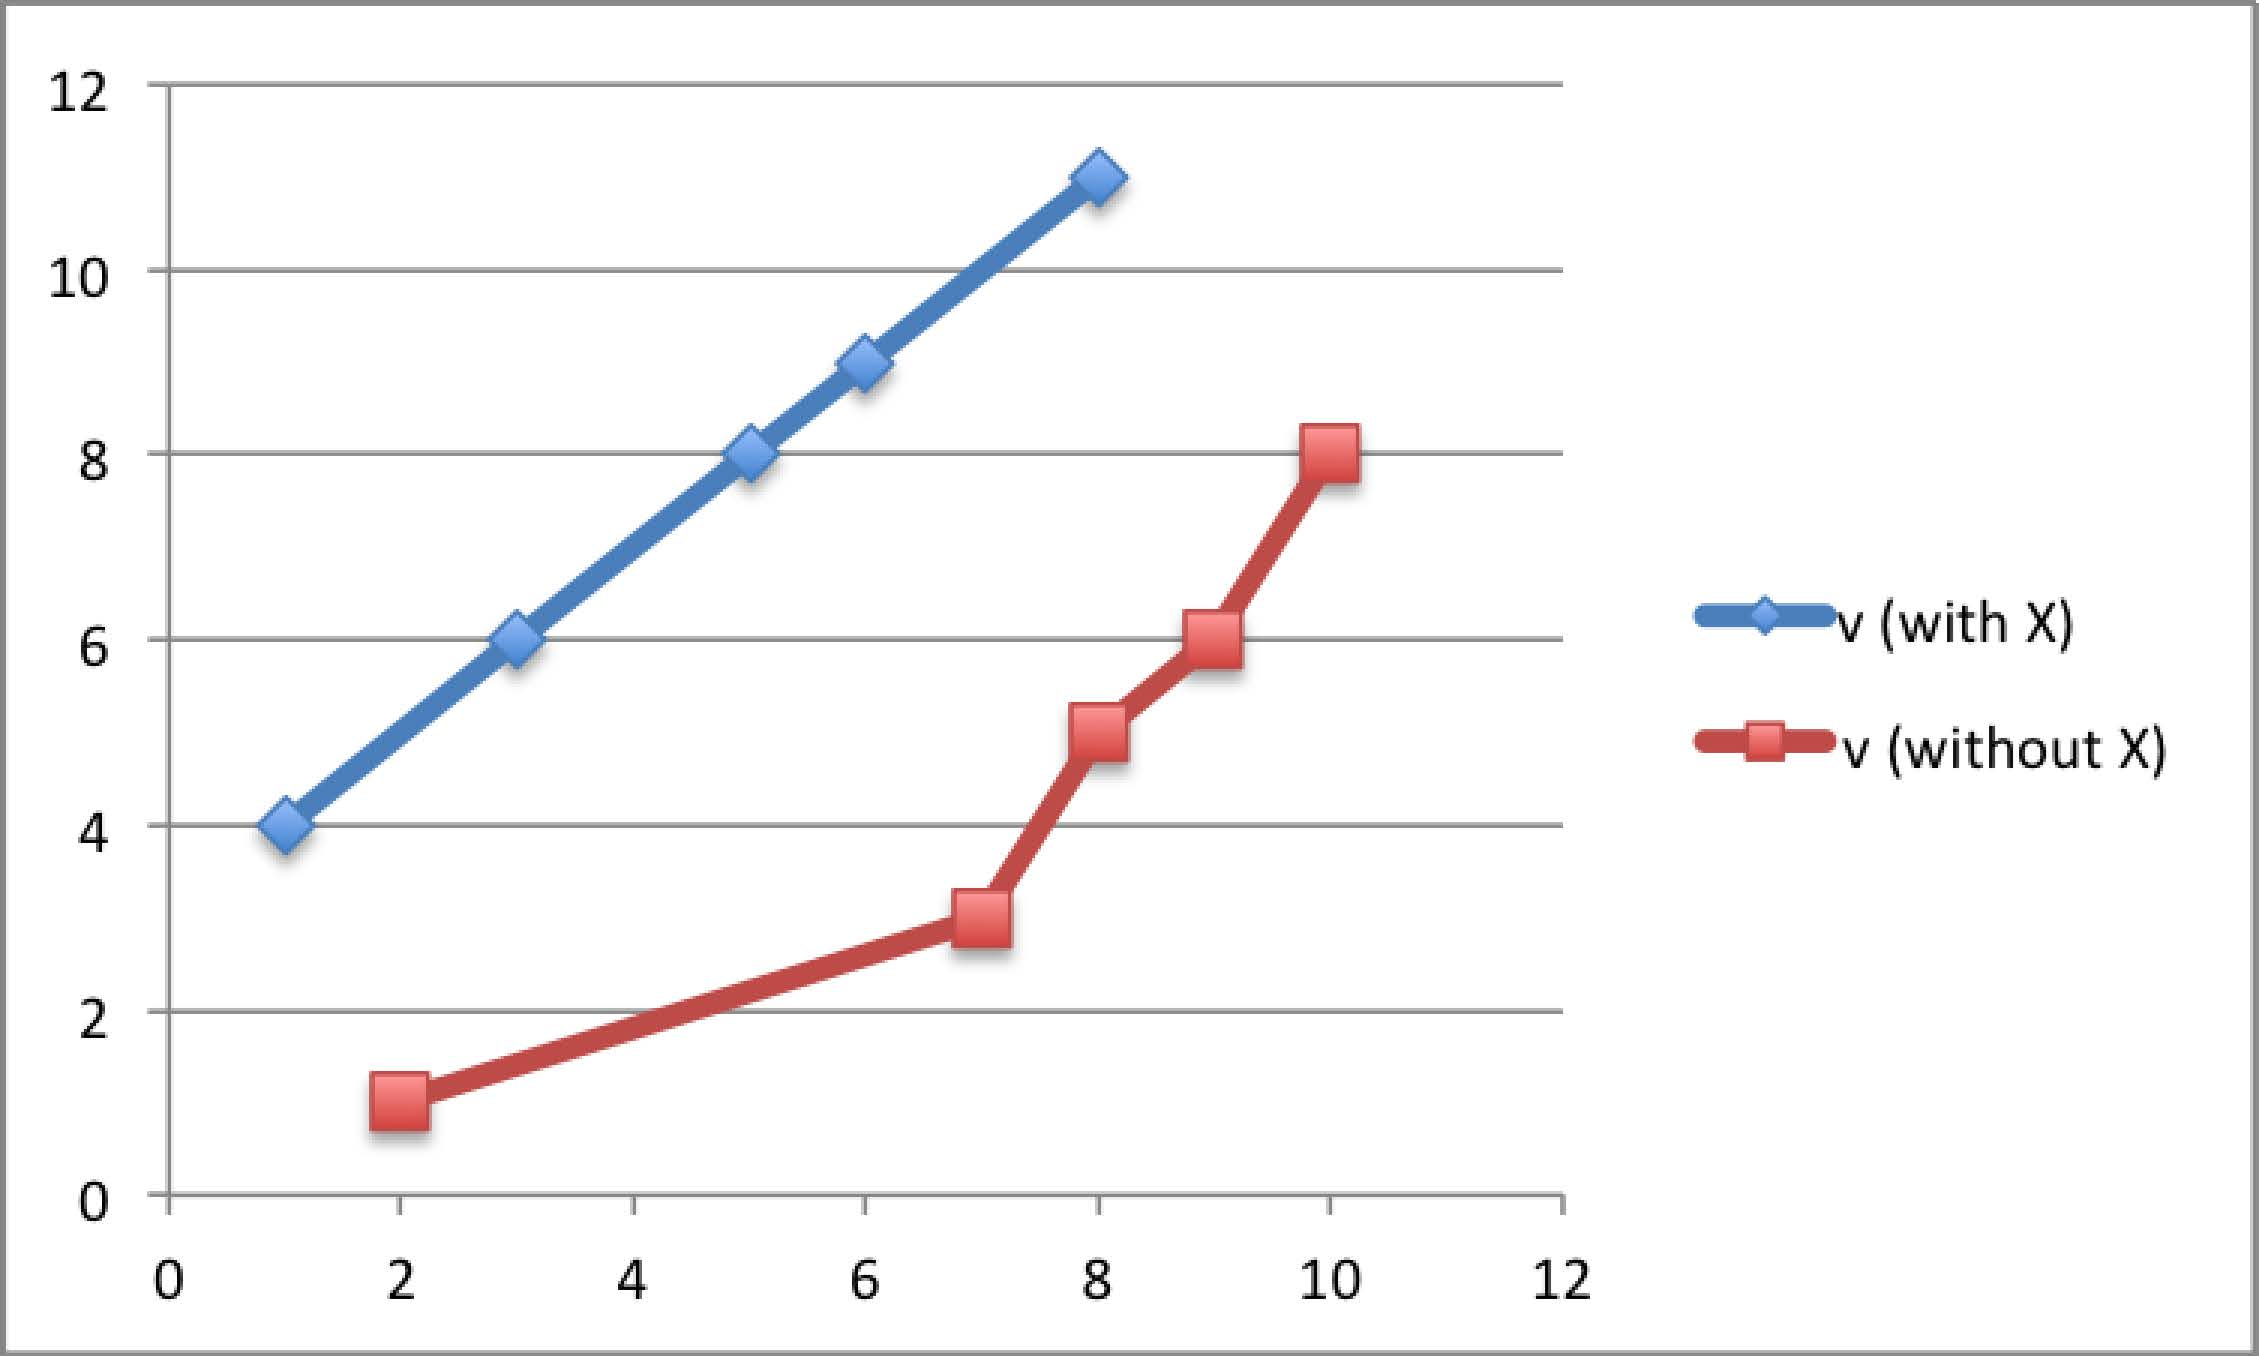
\includegraphics[scale=0.75]{RD}
    \caption{A sample graph image}
  \end{center}
\end{figure}

\subsection{Subfig test}

\begin{figure}[ht]
  \centering
  \subfloat[First fig.]{
    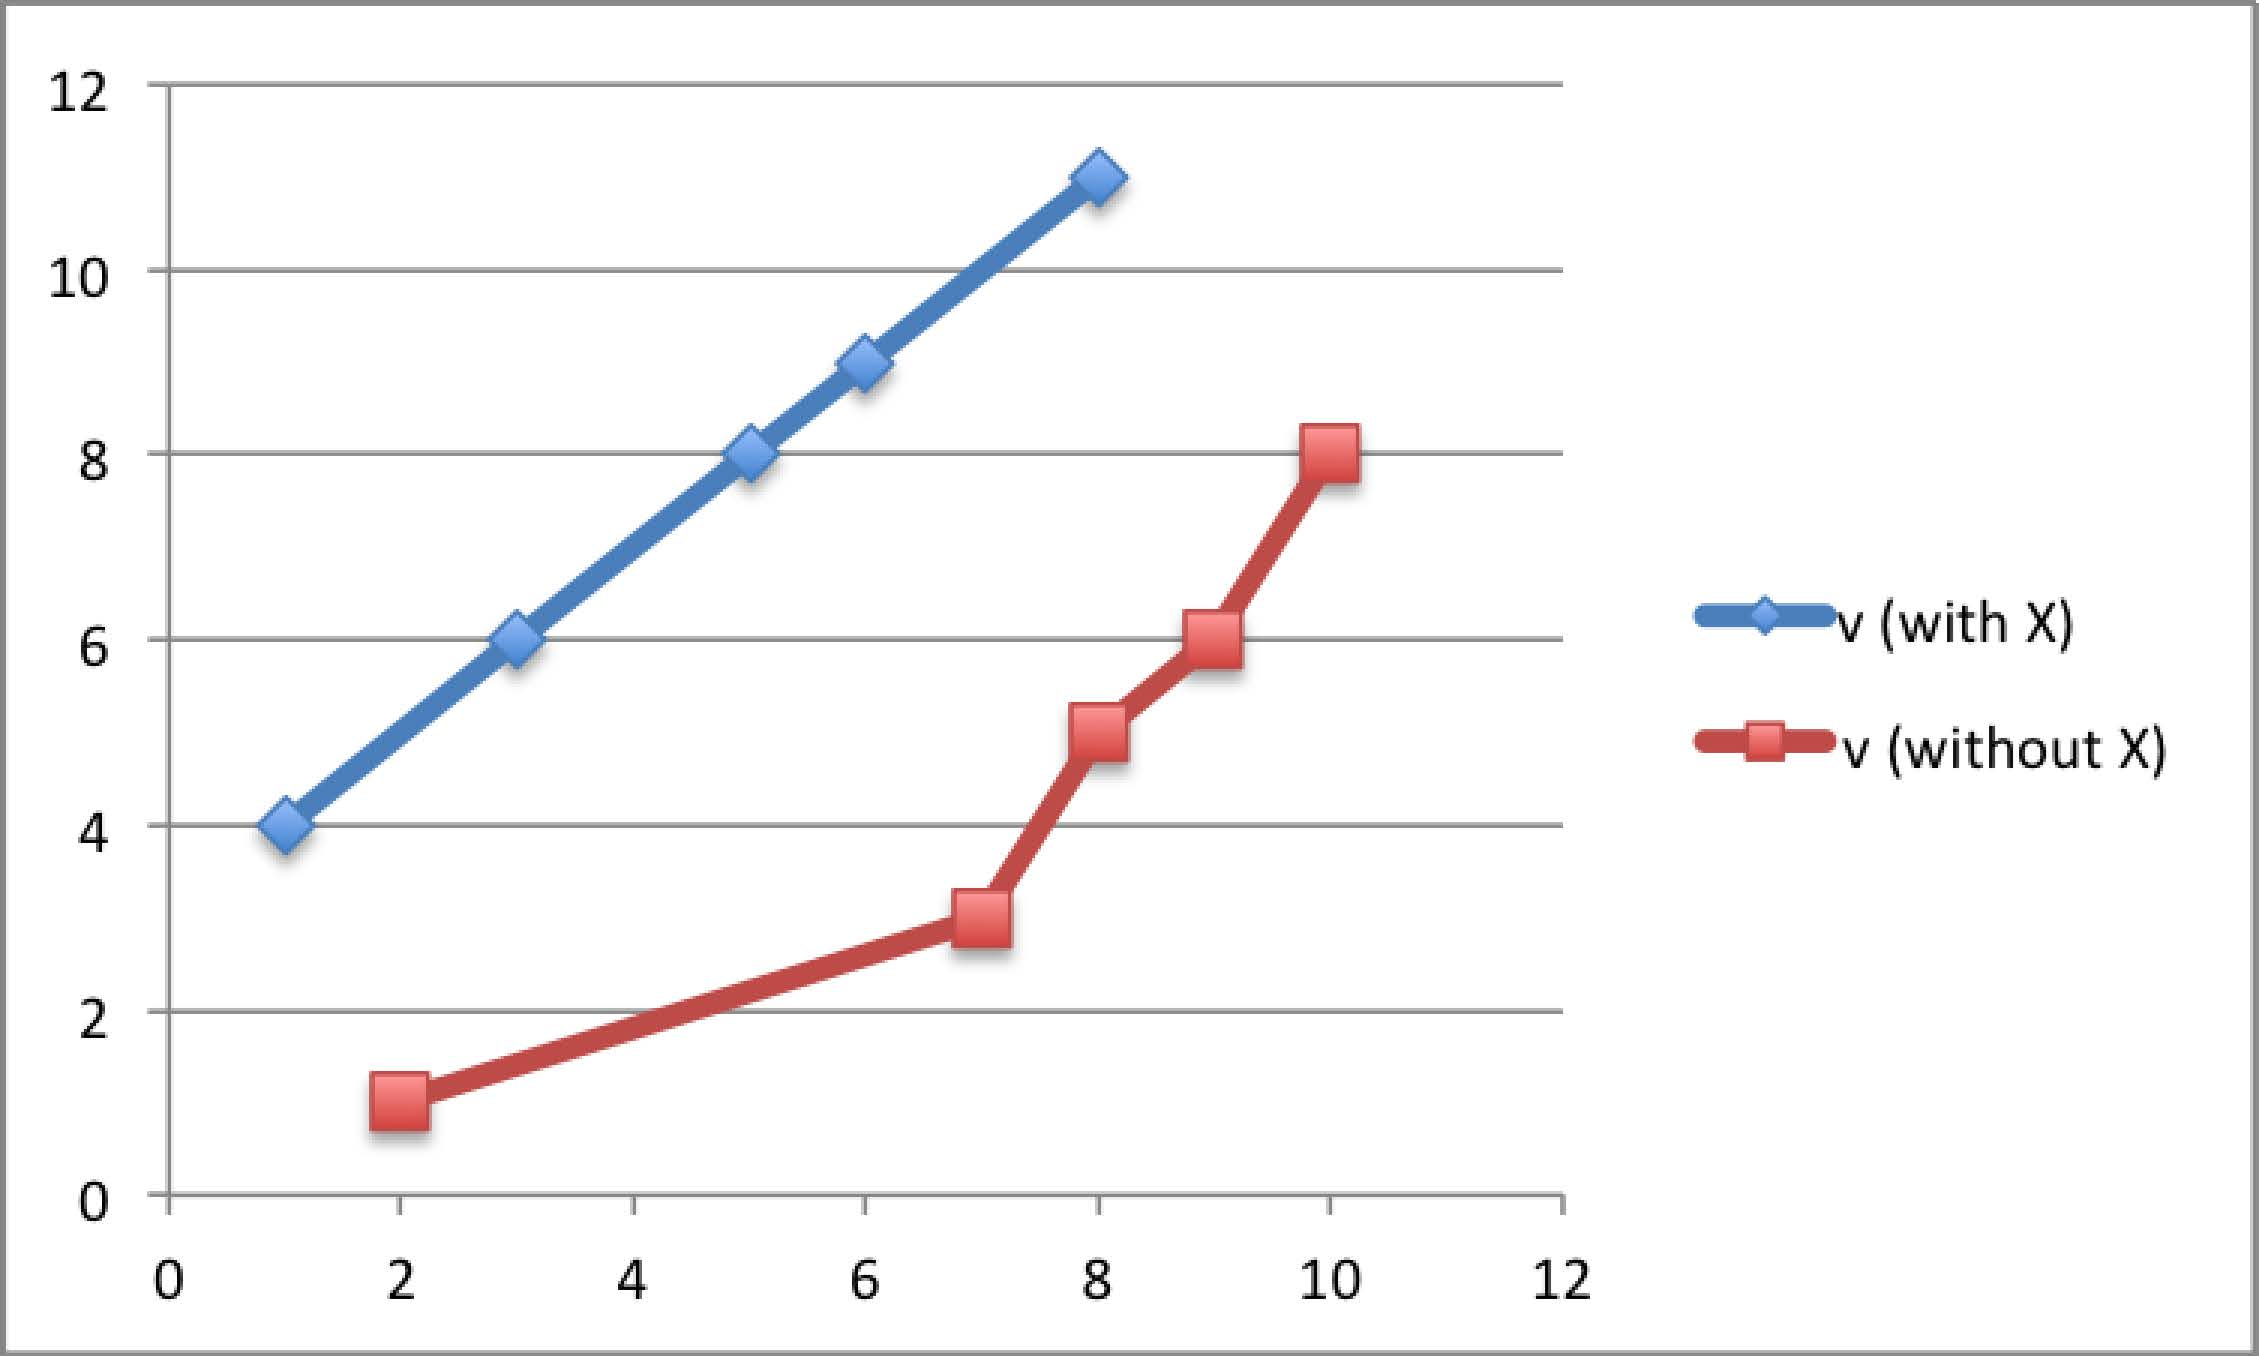
\includegraphics[width=0.45\columnwidth]{RD} \label{fig:two-figs:v1}
  }
  \subfloat[Second fig.]{
    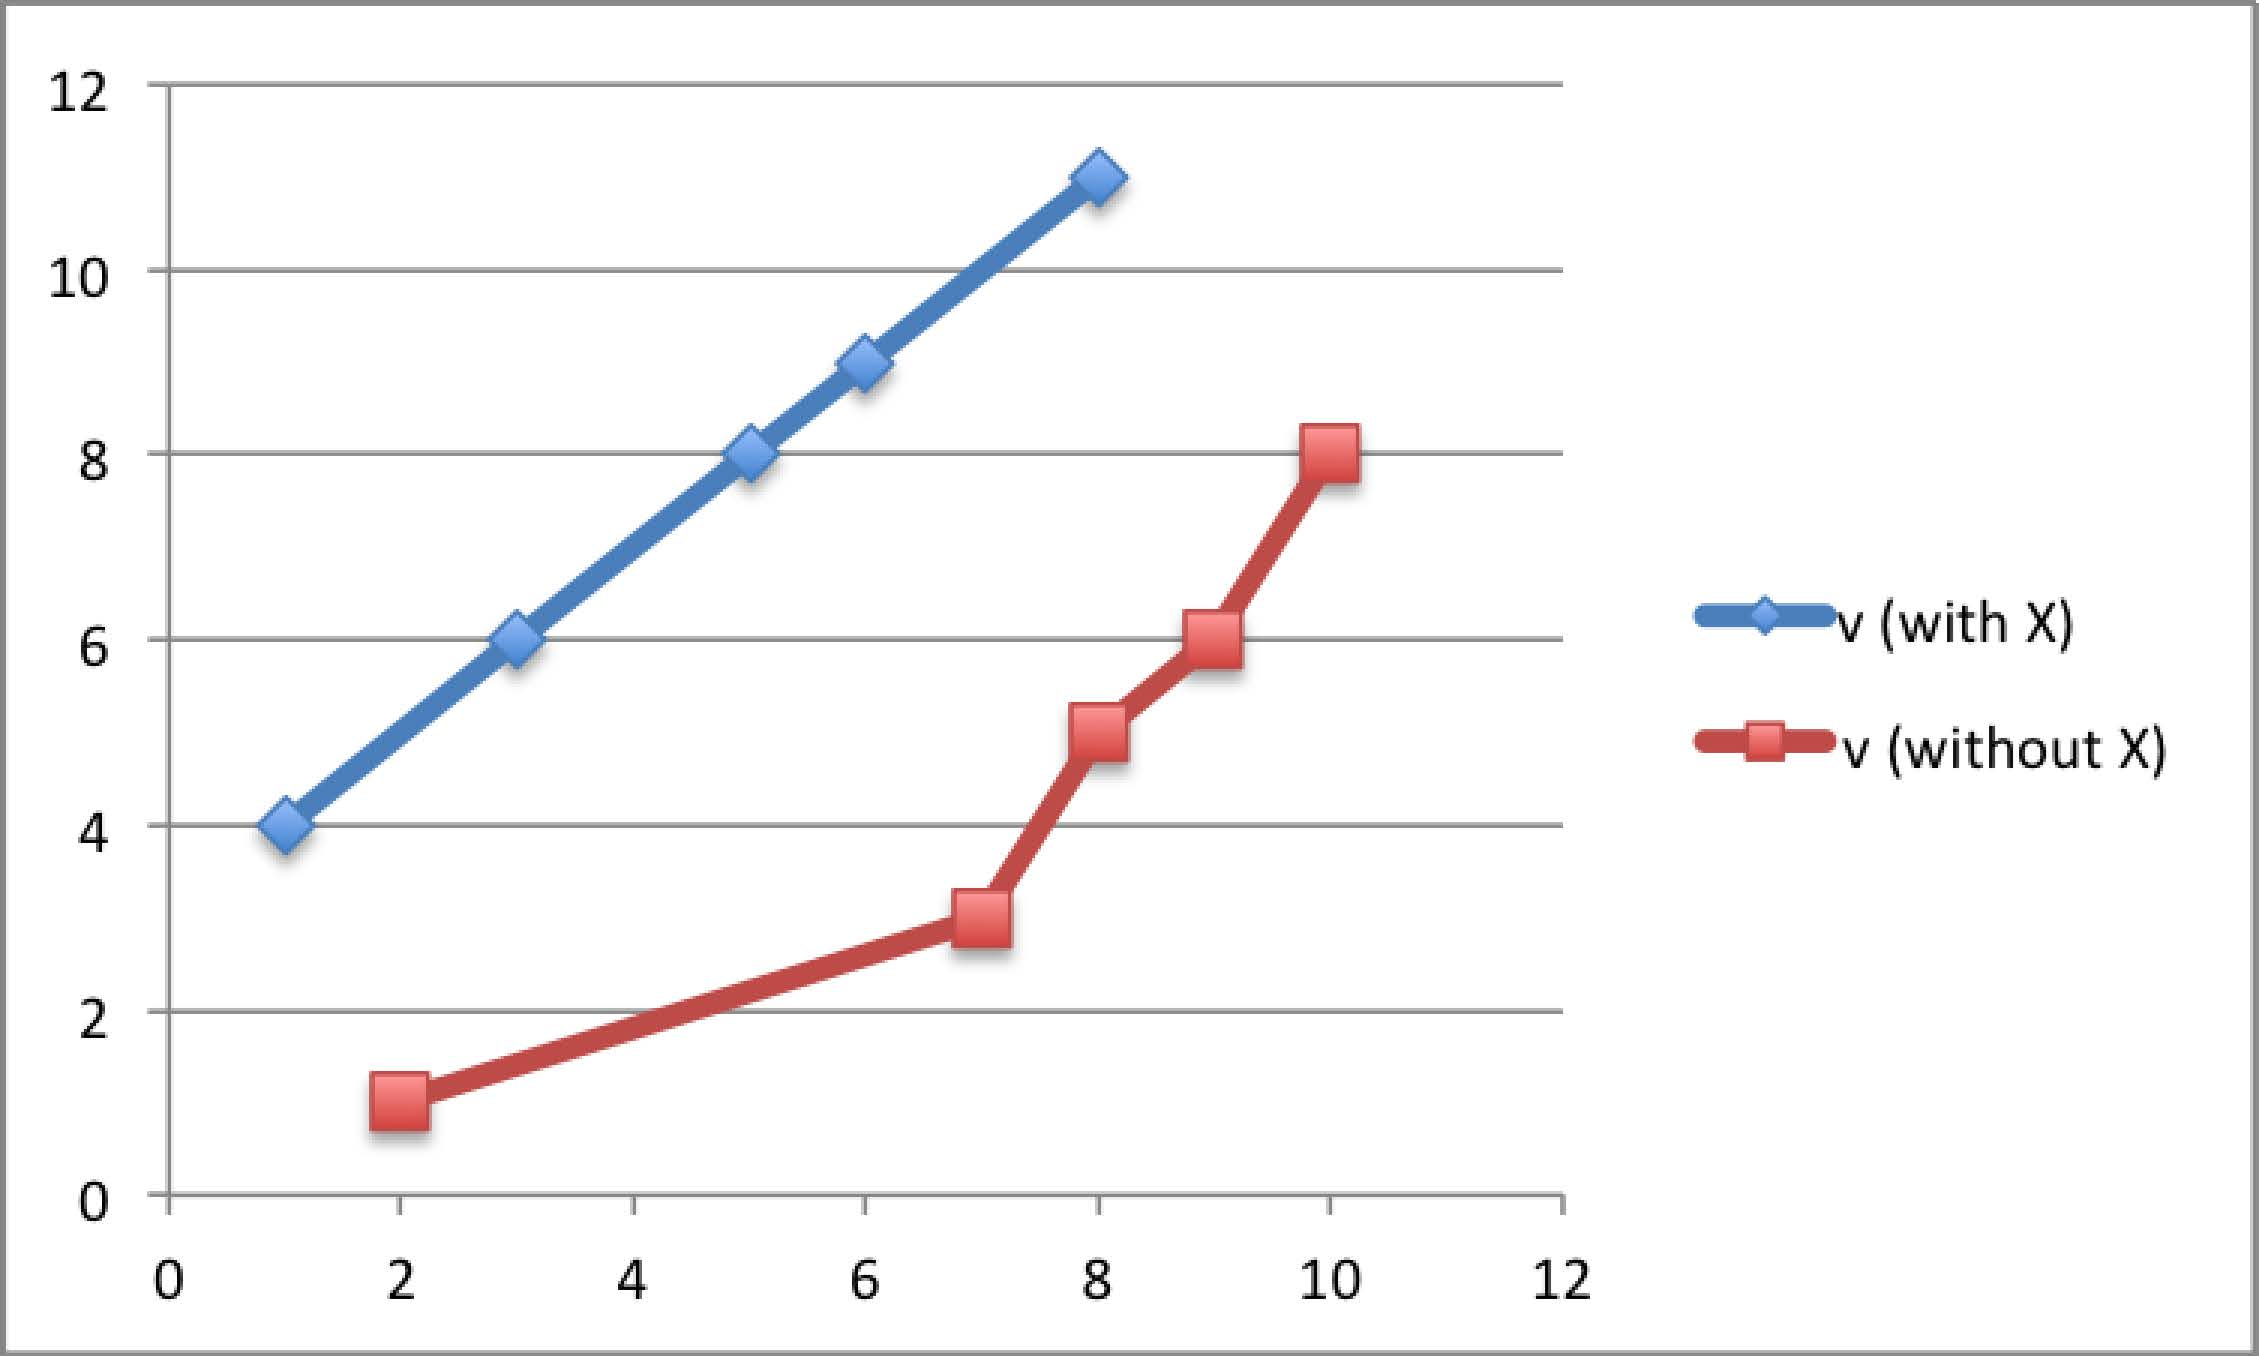
\includegraphics[width=0.45\columnwidth]{RD}
  }
  \caption{A sample of two sub figures. The two different figures are combines by the \texttt{subfloat} package. This figure has an extreme long caption for verifying whether the hanging paragraph of the single-spacing caption works. \label{fig:two-figs}}
\end{figure}

Try to ref \autoref{fig:two-figs}, and \autoref{fig:two-figs:v1}.

\subsection{Formulation test}
Test the following formulation:
\begin{subequations}
  \renewcommand{\theequation}
  {\theparentequation-\arabic{equation}}
  \begin{align}
    \frac{\partial \mathcal{L}(\mathbf{w},~b)}{\partial \mathbf{w}} &= \mathbf{w} + C \sum\limits_i\frac{\partial \ell_i}{\partial \mathbf{w}}, \label{fml:eq1:partialW}\\
    \frac{\partial \mathcal{L}(\mathbf{w},~b)}{\partial b} &= C \sum\limits_i\frac{\partial \ell_i}{\partial b}, \label{fml:eq1:partialb}
  \end{align}
\end{subequations}
where the gradients are used in support vector machine.

Try to refer the equations like this: \eqref{fml:eq1:partialb}.

\subsection{A Sample subsection}
It is a long established fact that a reader will be distracted by the readable content of a page when looking at its layout. The point of using Lorem Ipsum is that it has a more-or-less normal distribution of letters, as opposed to using 'Content here, content here', making it look like readable English \cite{gass}. Many desktop publishing packages and web page editors now use Lorem Ipsum as their default model text, and a search for 'lorem ipsum' will uncover many web sites still in their infancy. Various versions have evolved over the years, sometimes by accident, sometimes on purpose (injected humour and the like).

\begin{figure}[ht]
  \label{hourglass}
  \begin{center}
    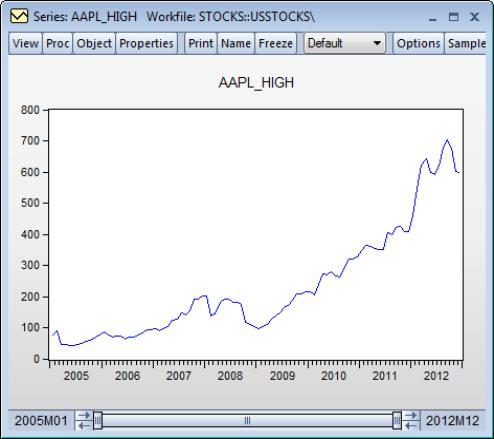
\includegraphics{graph}
    \caption{Another plot image}
  \end{center}
\end{figure}

\subsection{Another subsection} 
There are many variations of passages of Lorem Ipsum available, but the majority have suffered alteration in some form, by injected humour, or randomised words which don't look even slightly believable. If you are going to use a passage of Lorem Ipsum, you need to be sure there isn't anything embarrassing hidden in the middle of text. All the Lorem Ipsum generators on the Internet tend to repeat predefined chunks as necessary, making this the first true generator on the Internet. It uses a dictionary of over 200 Latin words, combined with a handful of model sentence structures, to generate Lorem Ipsum which looks reasonable. The generated Lorem Ipsum is therefore always free from repetition, injected humour, or non-characteristic words etc.

\cleardoublepage

\chapter{A New Section - Such as Related Work}
\label{cahp-rl}

Duis aliquam hendrerit nunc vitae euismod. Nam in laoreet ante. Vestibulum nec purus eget urna varius commodo luctus in lacus. Quisque eu nisl dui. Maecenas sagittis rutrum ante id imperdiet. Sed semper odio vel est bibendum commodo. Vivamus lacinia facilisis ante. Etiam venenatis at eros eu sollicitudin. Proin aliquet, neque in suscipit finibus, purus mi elementum est, finibus elementum libero turpis faucibus nibh. Proin orci arcu, euismod a lacinia vel, porta a turpis \cite{apples1}.

\section{The subsection -- about a Toolkit}

Praesent eget neque ac tortor finibus hendrerit et eu mauris. Nam quis finibus risus, ac tristique turpis. Curabitur non mauris eget sapien eleifend scelerisque lobortis eu lacus. Sed metus augue, volutpat id tristique in, ultrices in massa. Donec et dui in massa rhoncus scelerisque. Nunc luctus dui sed ullamcorper molestie. Phasellus efficitur nec est sit amet dignissim. In convallis orci ac urna maximus, et congue nisl lobortis.

\section{Internals of the toolkit}

Sed facilisis commodo leo, id interdum est. Vivamus ultricies pharetra tortor, nec imperdiet enim mattis non. Duis sagittis sem ut urna sodales semper. Vestibulum ullamcorper dui at libero faucibus vulputate at nec nulla. Fusce justo est, maximus eu commodo sed, sagittis dictum felis. Integer id velit ac ipsum volutpat bibendum. Nunc dictum pretium eros, tincidunt sodales enim porta a.

\begin{figure}[ht]
  \begin{center}
    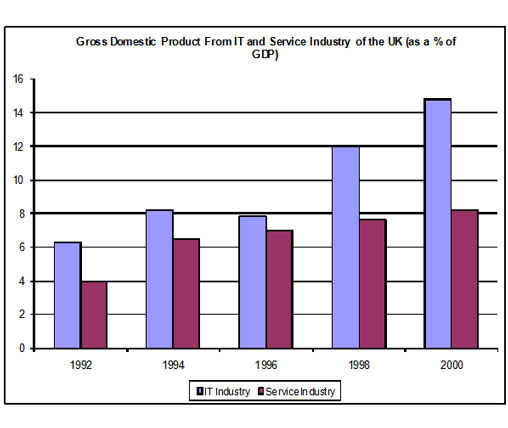
\includegraphics[scale=0.65]{Histogram}
    \caption{Some Bar Chart}
  \end{center}
\end{figure}

Another list can go like this, and more explanations can be added \cite{apples2}.
\begin{enumerate}
  \item
  Connectivity protocols 
  \item
  Resource protocols 
  \item
  Collective protocols 
\end{enumerate}

\section{Services and Technologies}
Vestibulum tempus ipsum in gravida hendrerit. Donec vehicula mi a rhoncus pellentesque. Morbi sit amet vestibulum tortor. Nulla facilisi. Nulla felis velit, accumsan maximus ornare sit amet, congue a dolor. Mauris quis pulvinar justo. Phasellus nec consequat tellus. Ut tempor venenatis risus. Nam sit amet mauris tincidunt leo porttitor tempor. Nam at urna ac leo fringilla accumsan. Morbi eu tristique ligula. Cras ut pellentesque orci. Orci varius natoque penatibus et magnis dis parturient montes, nascetur ridiculus mus. Duis suscipit nunc diam, vitae semper nibh maximus rhoncus. Donec pharetra elit viverra sapien elementum aliquet. Duis hendrerit quam elit, in pretium enim ultricies ac.

\subsection{An example for sub-sub-section}
Etiam risus ante, viverra vel diam sed, eleifend blandit quam. Vivamus quis gravida arcu. Fusce ac est ut velit maximus pellentesque vitae quis massa. Aenean eget tortor nisi. Phasellus hendrerit nibh sit amet dolor molestie interdum vel a lacus. Nam est leo, consequat id nibh ac, molestie facilisis velit. Cras at urna nisl.

\section{Programming Section}

Praesent in feugiat turpis, et laoreet turpis. Etiam lobortis, metus sit amet iaculis tincidunt, velit orci porta magna, vitae faucibus arcu orci nec justo. Morbi quis elit non massa tincidunt ornare ullamcorper quis mauris. Vivamus nec sollicitudin tortor, venenatis cursus mi. Donec at turpis non leo euismod hendrerit vulputate et tortor. Quisque malesuada lectus vitae orci condimentum sagittis. Nunc ut ligula a eros venenatis pretium

\begin{center}
  \begin{parbox}[t]{.45\linewidth}
    {\textsf{\underline{Sample Mathematical Explanation} \\
      (1) P $\xrightarrow{getPK(R)}$ GSM$_u$ \\
      1.1 $GSM_u$ $\xrightarrow{R}$ GSM$_R$\\
      1.2 $GSM_u$ $\xleftarrow{PK_R}$ GSM$_R$\\
      (2) P $\xleftarrow{PK_R}$ $GSM_u$ \\
      (3) P $\xrightarrow{C=Enc_{PK_R}(M)}$ R \\
      (4) P $\xleftarrow{M}$ R \\
      (5) P considers R authenticated \\
      \hfill
    }} \\
  \end{parbox}
\end{center}

\cleardoublepage

\chapter{Conclusions}
\label{chap-conclusion}
In odio metus, pellentesque vitae tellus sed, bibendum cursus tortor. Vestibulum nec nunc non felis aliquet luctus vitae porta massa. Cras eu venenatis odio, cursus ultricies purus. Vestibulum ac blandit nibh, vitae porttitor ipsum. Nullam vestibulum sagittis metus, ut rutrum est vehicula non. Duis interdum tempor est non posuere. Curabitur metus mauris, elementum sit amet augue a, sollicitudin sodales arcu.

Nulla congue at odio egestas fringilla. Quisque sollicitudin ante non sem facilisis pharetra. Vivamus ut augue gravida, suscipit augue quis, eleifend augue. Sed finibus finibus magna quis luctus. Cras cursus, nisl in commodo venenatis, neque ipsum interdum sem, at venenatis lacus dolor vel mauris. Etiam elementum nibh tristique justo pellentesque, ut pulvinar dolor dictum. Pellentesque habitant morbi tristique senectus et netus et malesuada fames ac turpis egestas. Aenean non ligula ac justo consequat aliquet. Maecenas rhoncus sapien nec justo condimentum, ac varius lacus ullamcorper. Aliquam erat volutpat. Etiam posuere justo a eleifend porttitor. Nulla eu elit pellentesque, feugiat metus nec, fringilla ligula. Ut nibh lorem, tempus at convallis sed, pharetra at metus. Curabitur id purus porttitor, ultricies tortor a, tincidunt ligula. Mauris felis elit, sodales ac sollicitudin id, tincidunt a quam.

\cleardoublepage

%\begin{thebibliography}{10}
%\bibitem{gridftp}W. Allcock, J. Bester, J. Bresnahan, A. Chervenak, I. Foster, C. Kesselman, S. Meder, V. Nefedova, D. Quesnel, and S. Tuecke, "Data Management and Transfer in High-Performance Computational Grid Environments," Proceedings of the 9th International Conference on Grid Computing, 2010, Chicago, IL, USA, June 2010.
%
%\bibitem{gass}J. Bester, I. Foster, C. Kesselman, J. Tedesco, S. Tuecke, "GASS: A Data Movement and Access Service for Wide Area Computing Systems," Sixth Workshop on I/O in Parallel and Distributed Systems, May 5, 1999.
%
%\bibitem{apples1}F. Berman, R. Wolski, S. Figueira, J. Schopf, G. Shao, "Application-Level Scheduling on Distributed Heterogeneous Networks," Proceedings of Supercomputing, 1996.
%
%\bibitem{apples2}F. Berman and R. Wolski, "The AppLeS Project: A Status Report ", Proceedings of the 8th NEC Research Symposium, Berlin, Germany, May 1997.
%\end{thebibliography}

% \bibliographystyle{acm}  % ACM style is not recommended by ECE
\bibliographystyle{IEEETrans}  % IEEE style is recommended by ECE
\bibliography{bib/ref}

\end{document}
